\documentclass[11pt]{article}
\usepackage[margin=2cm]{geometry}
\usepackage{graphicx}
\usepackage[dvipsnames]{xcolor}
\pagenumbering{gobble}
\graphicspath{{img}}


\begin{document}

\title{Emulator Video/Input Integration Documentation Imagination Revelation Deliberation}
\author{Oliver Killane}
\date{10 June 2021}

\maketitle

    \section*{Memory Layout}
        \begin{center}
            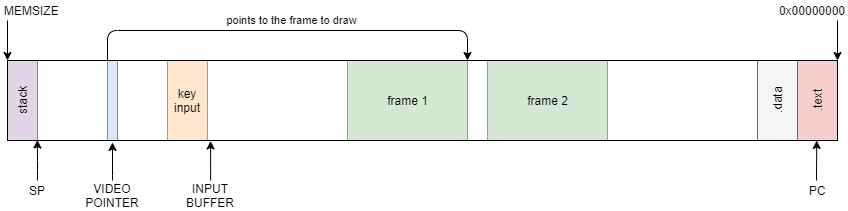
\includegraphics[width=\textwidth]{memory layout}
        \end{center}
        \centerline{\textbf{Fixed memory locations}}
        \begin{tabular}{r p{7cm} p{7cm}}
            Location & Use & Reasoning \\
            \hline
            VIDEO POINTER & Points to start of current frame to Display. & Allows for multiple buffers, without extra instructions or additions to the asm. \\
            INPUT BUFFER & A buffer containing 64 bytes, each byte storing a keyboard event. & Program can read buffer, clear buffer, emulator refill. \\
        \end{tabular}
    
    \section*{Input Buffer}
        \begin{center}
            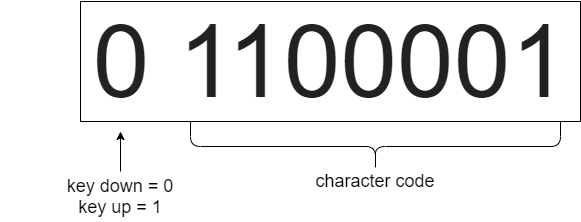
\includegraphics[width=6cm]{key input storage}
            \begin{tabular}{c c c}
                SDL Key & Key & Value \\
                \hline
                SDLK\_0$\to$9 & 0$\to$9 & 48 $\to$ 57 \\
                SDL\_ESC & escape & 27 \\
                SDL\_a$\to$z & a $\to$ z & 97 $\to$ 122 \\
                SDL\_UP & up arrow & 1073741906 \\
                SDL\_DOWN & down arrow & 1073741905 \\
                SDL\_LEFT & left arrow & 1073741904 \\
                SDL\_RIGHT & right arrow & 1073741903 \\
                SDL\_ENTER & enter key & 13 \\
            \end{tabular}
        \end{center}
        To keep each to 8 bytes, we will use ascii EOT (4), ENQ (5), ACK (6) and BEL (7) for up, down, left and right arrow keys.
        \begin{center}
            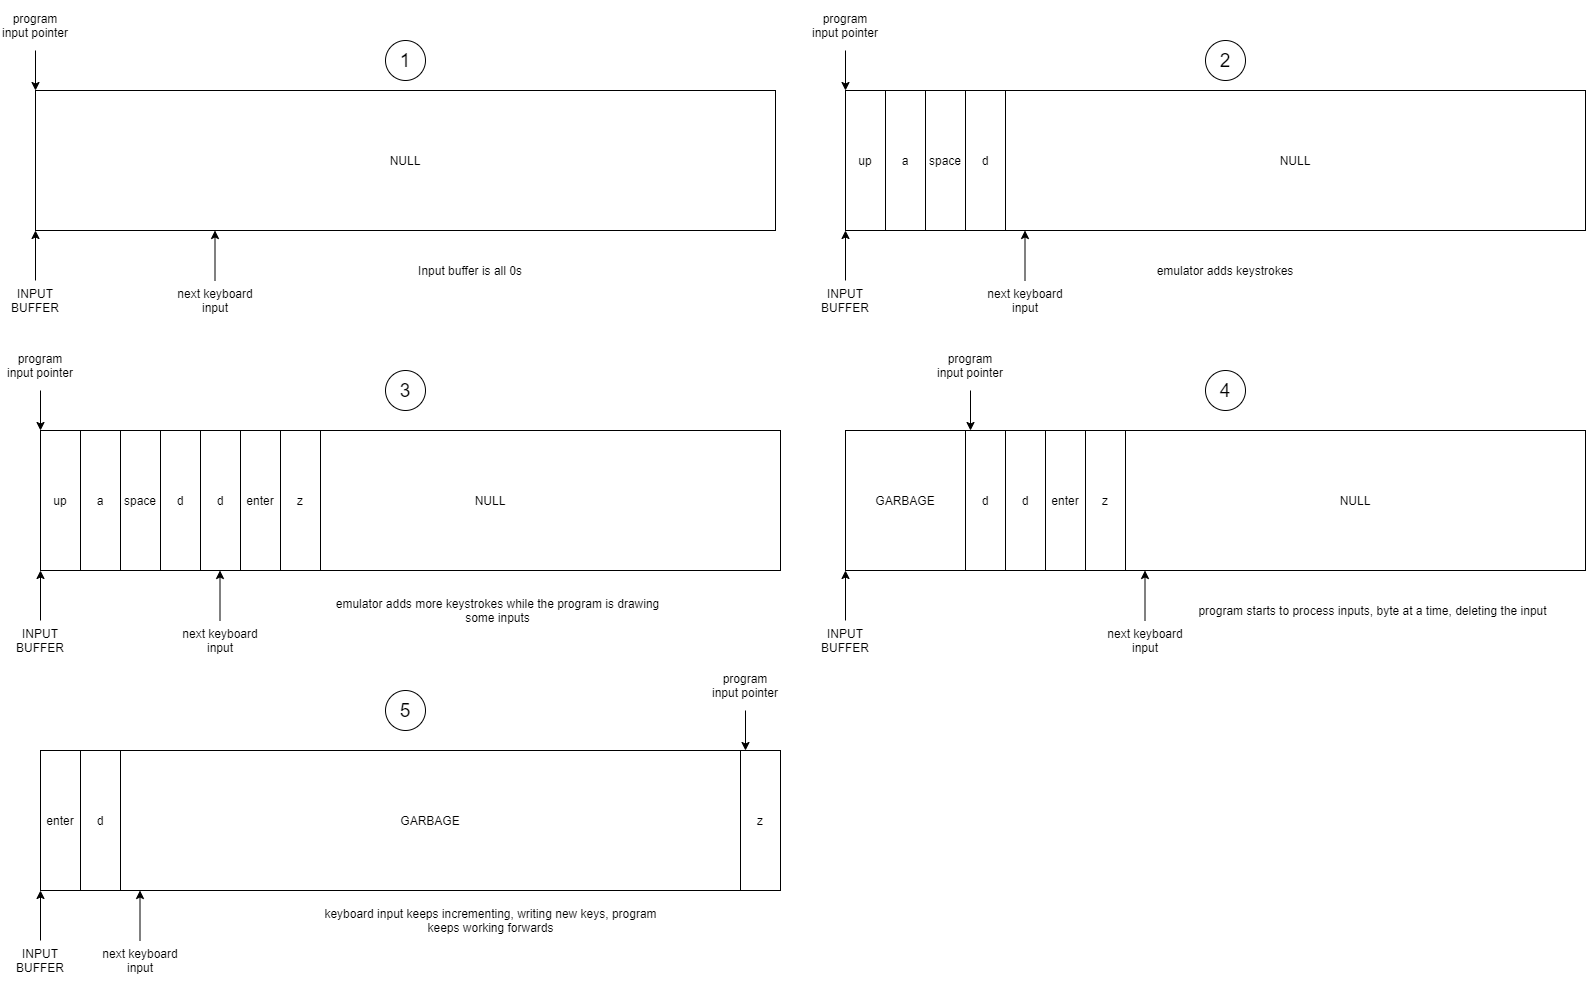
\includegraphics[width = \textwidth]{key input queue}
        \end{center}
\end{document}

